\chapter{Audience and Summary}

\newthought{Welcome to MSAN501}, the computational analytics boot camp at the University of San Francisco! This exercise book collects all of the labs you must complete by the end of the boot camp in order to pass.  The labs start out as very simple tasks or step-by-step recipes but then accelerate in difficulty, culminating with an interesting text analysis project. You will build all projects in Python (2.7.x).

\marginnote[-1in]{As you progress through these exercises, you'll learn a great deal about Python and the following libraries: {\tt matplotlib}, {\tt numpy}, {\tt scipy}, and {\tt py.test}. You'll also learn how to run jobs on computers in the cloud.}

This course is specifically designed as an introduction to analytics programming for those who are not yet skilled programmers. The course also explores many concepts from math and statistics, but in an empirical fashion rather than symbolically as one would do in a math class. Consequently, this course is also useful to programmers who'd like to strengthen their understanding of numerical methods.

\marginnote[-1in]{
\begin{center}
\scalebox{.65}{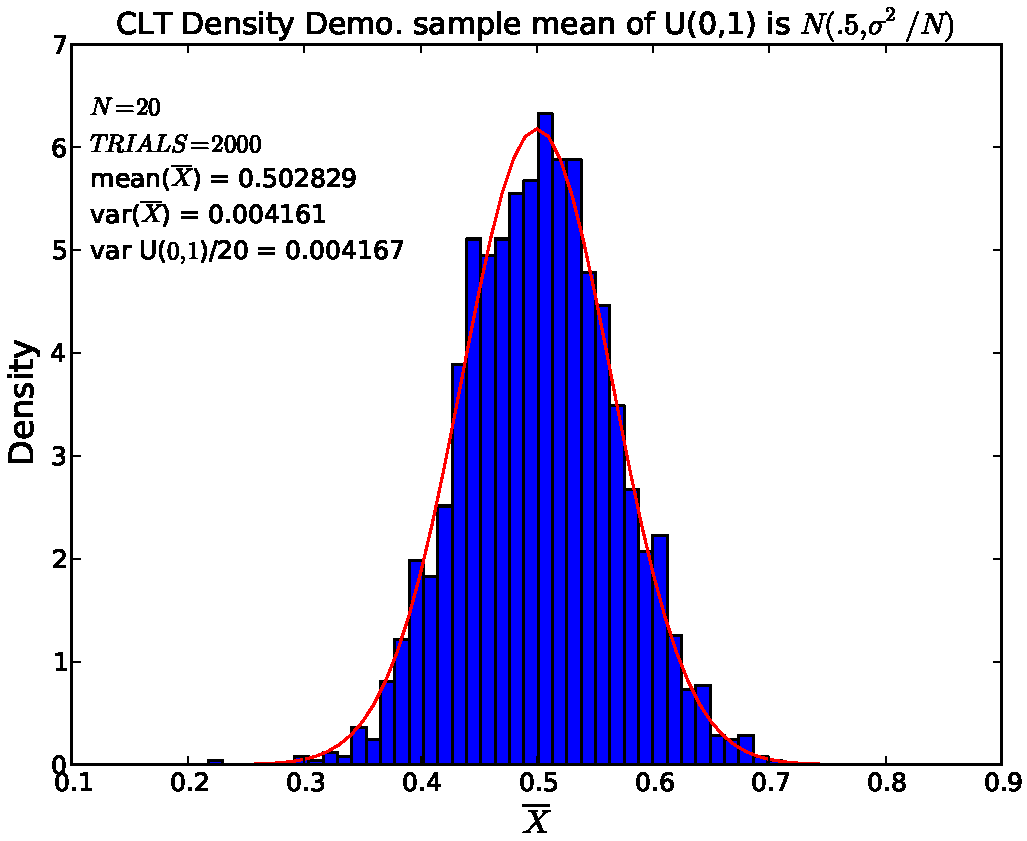
\includegraphics{figures/clt_unif-2000-20.pdf}}
\scalebox{.65}{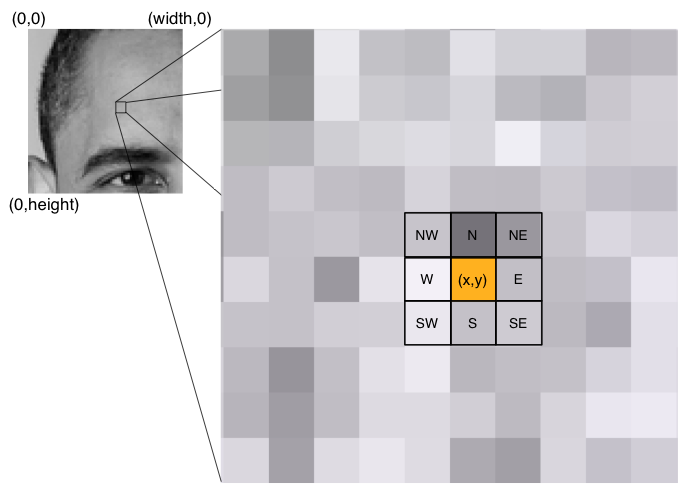
\includegraphics{figures/region.png}}\\
\scalebox{.35}{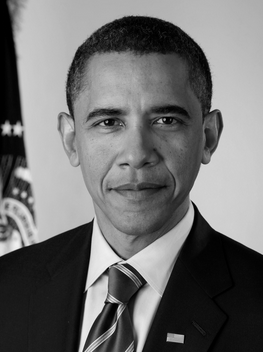
\includegraphics{figures/obama.png}}
\scalebox{.35}{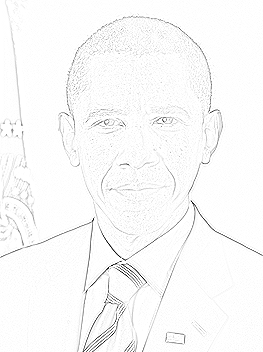
\includegraphics{figures/obama-negative-edges}}
\scalebox{.65}{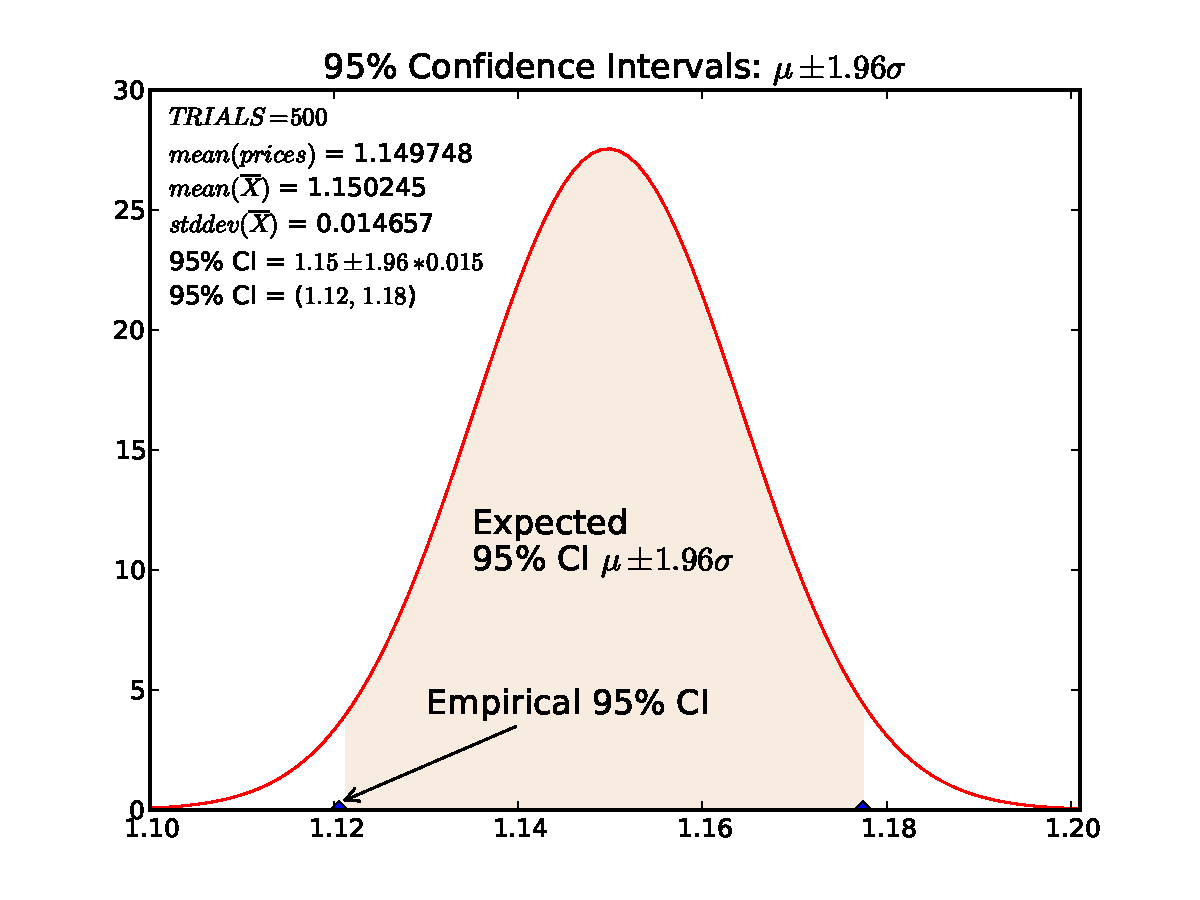
\includegraphics{figures/conf-500.pdf}}
\scalebox{.65}{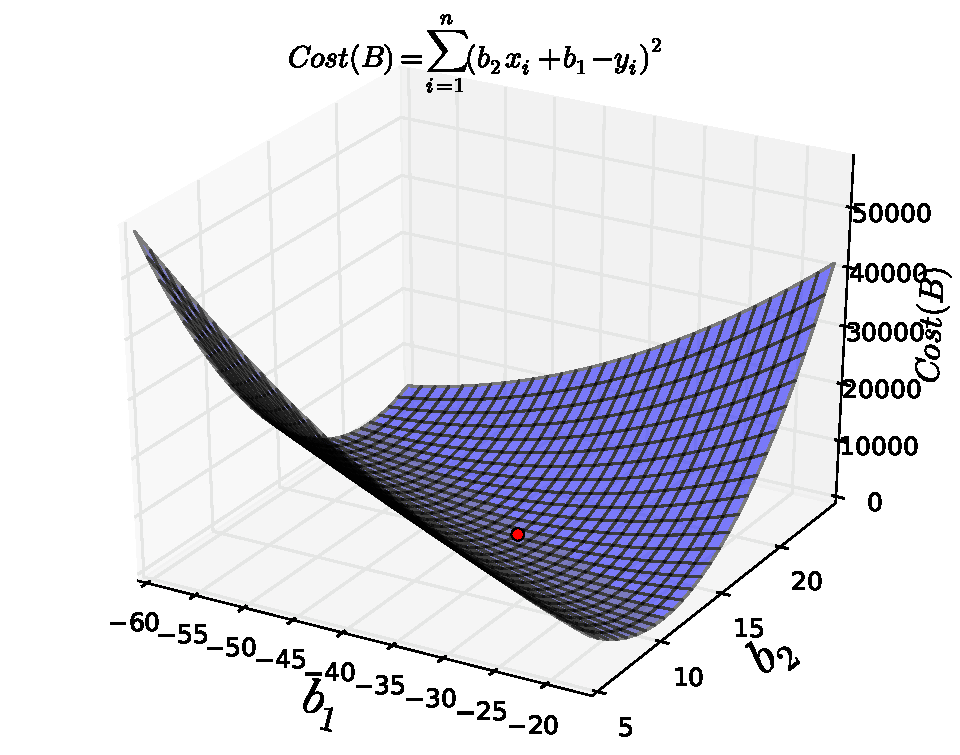
\includegraphics{figures/wage-murders-cost-3d.pdf}}
\scalebox{.65}{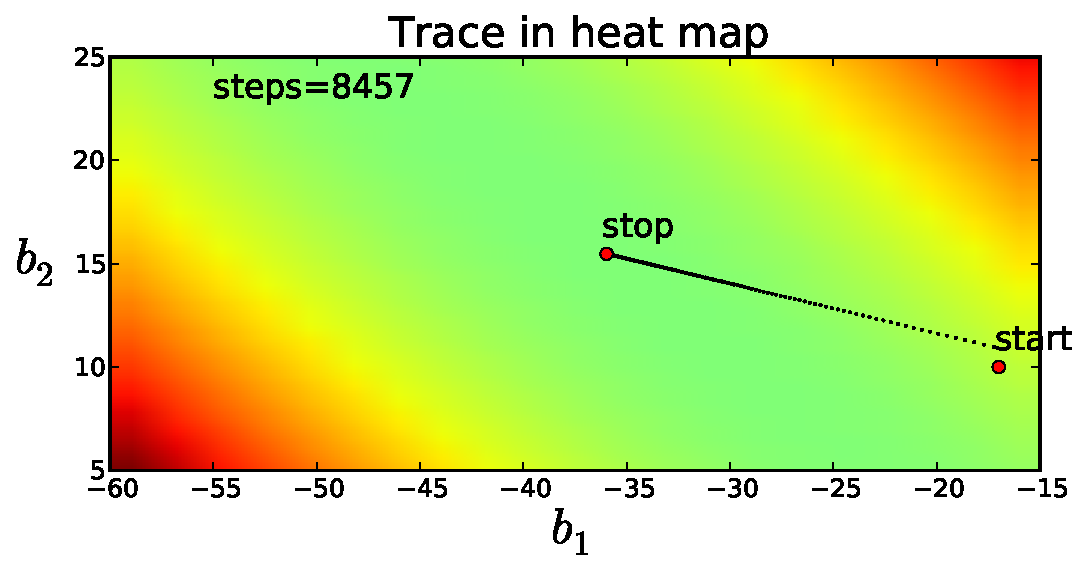
\includegraphics{figures/wage-murders-heatmap-trace1.pdf}}
\end{center}
}

The exercises are grouped into multiple parts. We begin by looking at our fundamental tools, such as the command line and PyCharm. Then we'll study how computers represent data and images, learn simple data structures, and build some visualizations. Next, we'll study how to solve a number of math and statistics problems related to analytics. The empirical statistics part strives to give an intuitive feel for random variables, density functions, the central limit theorem, hypothesis testing, and confidence intervals. It's one thing to learn about their formal definitions, but to get a really solid grasp of these concepts, it really helps to observe statistics in action. All of the techniques we'll use in empirical statistics rely on the ability to generate random values from a particular distribution. We can do it all from a uniform random number generator.

The next set of exercises deal with function optimization. Given a particular function, $f(x)$, optimizing it generally means finding its minimum or maximum, which occur when the derivative goes flat: $f'(x) = 0$. When the function's derivative cannot be derived symbolically, we're left with a general technique called {\em gradient descent} that searches for minima.

Next, you'll get an introduction to text analysis. We will compute something called {\em TFIDF} that indicates how well that word distinguishes a document from other documents in a corpus.  That score is used broadly in text analytics.

Finally, we'll launch some machines in the cloud and perform some small distributed computing tasks using hadoop and Python.

\chapter{Grading}

You will be using {\tt github.com} to submit your projects (and we'll learn more about {\tt git} shortly).  Once you have completed the tasks and they pass any test files I've provided, you will notify me that projects are ready for grading adding a ``tag'' to your repository.  I will review your code and make sure that it passes the tests. Usually I will have some comments and commit changes and comments back to the repository. You must fix all of that and notify me by adding another tag to your repository. Once you have passed, I will add a tag to let you know it has been graded.

This class is pass/fail and all of the projects are pass/fail. You simply have to get past the tests and my code review for each exercise in this book.

Here are the tags that you are to enter when you complete each task:

\begin{description}
\item[hist] Histograms Using matplotlib
\item[images] Image Processing
\item[graphs] Graph Adjacency Lists and Matrices
\item[stats] All exercises in Empirical statistics
\item[descent] Iterative Optimization Via Gradient Descent
\item[regression] Predicting Murder Rates With Gradient Descent
\item[tfidf] Summarizing Reuters Articles with TFIDF
\end{description}

I will tag the repository with {\tt pass }{\em X} for your tag {\em X}. For repeated submissions of {\em X}, use {\em X2}, {\em X3} etc...